\documentclass{article}
\usepackage{enumerate}
\usepackage{amsmath}
\usepackage{caption}
\usepackage[hidelinks]{hyperref}
    \usepackage{graphicx}

  \usepackage[english]{babel}
  \usepackage[utf8]{inputenc}


\begin{document}
        \pagenumbering{roman}

      \begin{titlepage}
    \centering
    	{\scshape\LARGE FAMU-FSU College of Engineering \par}
    	\vspace{0.75cm}
    	{\scshape\large Department of Electrical and Computer Engineering\par}
    	\vspace{0.25cm}
      {\scshape\large\bfseries EEL3112L – Advanced Circuits with Computers Lab  \par}
      \vspace{0.25cm}
    	{\scshape\large \textit{ Spring 2017 Semester} \par}
    	\vspace{1.2cm}
      {\Large\bfseries DC Circuits I: Voltage, Current, Resistance, Ohm’s Law, and Electric Power \par}
      \vspace{1cm}
      \vfill
      \def\arraystretch{2.5}
      \begin{tabular}{  l  r  }
        \hline

          {\large\textbf{Lab Number:} }  & { \large 1 } \\ \hline
          {\large\textbf{Section:} }  & { \large 1 } \\ \hline
          {\large\textbf{Name:} }  & { \large Henry Troutman } \\ \hline
          {\large\textbf{Partner:} }  & { \large Ross Fleming } \\ \hline
          {\large\textbf{Instructor:} }  & { \large Dr. Petru Andrei } \\ \hline
          {\large\textbf{Assistant:} }  & { \large Ifedayo Ogundana } \\ \hline
          {\large\textbf{Date:} }  & { \large \today } \\ \hline

        \end{tabular}
        \vspace{3cm}

  \end{titlepage}


        \clearpage
    \newpage
    \tableofcontents
    \listoftables
    \listoffigures
    \newpage
    \pagenumbering{arabic}
    
  \section{Overview}
  \label{sec:Overview}
    \clearpage

  \section{Analysis}
  \label{sec:Analysis}
    \clearpage

  \section{Experimental Evidence}
  \label{sec:Experimental Evidence}
  
\subsection{Relevant Circuit Schematics}
\label{sub:Relevant Circuit Schematics}
  \begin{figure}[!ht]
  \centering
  \caption{Schematic for Verifying Ohm's Law\label{fig:ohmschem}}
  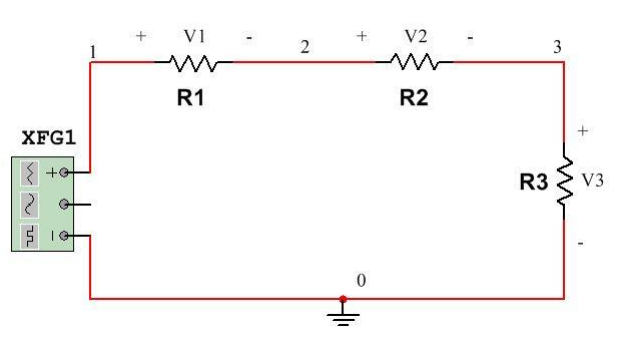
\includegraphics[width=0.75\textwidth]{img/c1.png}
  \end{figure}

  \begin{figure}[!ht]
  \centering
  \caption{Schematic for Measuring Maximum Power Transfer\label{fig:maxpowerschem}}
  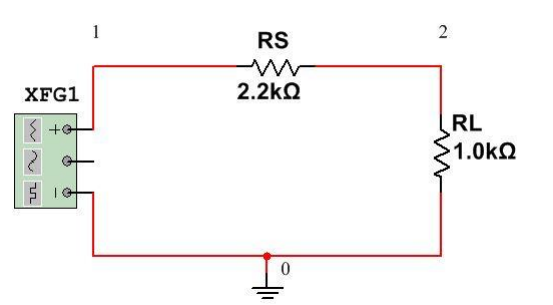
\includegraphics[width=0.75\textwidth]{img/c2.png}
  \end{figure}


\clearpage

\subsection{Results}
\label{sub:Results}

      \begin{table}[!ht]
  \captionsetup{font=large}
  \centering
  \caption{ List of Resistors Used }
  \label{tab: resultResistors }
  \begin{tabular}{   | l | c | c | c | r | }
  \hline

      Resistor &     Color Code &     Calculated Value ($ k \Omega $) &     Measured Value ($ k \Omega $)     \\ \hline
      1 &    Brown Black Red Gold &     1 &     0.99     \\ \hline
      2 &    Red Red Red Gold &     2.2 &     2.18     \\ \hline
      3 &    Brown Black Brown Gold &     0.1 &     0.099     \\ \hline
      4 &    Blue Blue Red Gold &     6.8 &    6.8     \\ \hline
      5 &    Brown Black Black Gold &     0.01 &     0.01     \\ \hline
      6 &    Orange Orange Red &     3.3 &    3.25     \\ \hline
      7 &    Brown Green Red Gold &     1.5 &    1.46     \\ \hline
      8 &    Yellow Purple Black Gold &     0.047 &     0.046     \\ \hline
      9 &    Orange White Black Gold &     0.039 &     0.039     \\ \hline
      10 &    Red Purple Black Gold &     0.027 &     0.027     \\ \hline
      11 &    Red Black Black Brown Brown &     2 &     2      \\ \hline
  
  \end{tabular}
  \end{table}



        
      \begin{table}[!ht]
  \captionsetup{font=large}
  \centering
  \caption{ Verification of Ohm's Law using resistor $R_1$ }
  \label{tab: ohm1 }
  \begin{tabular}{   | l | c | c | r | }
  \hline

      Source Voltage ($V_s$) &     $V_{R1}$ (V) &    $I_{R1}$ (mA)     \\ \hline
      0 &    0.0 &    0     \\ \hline
      0.5 &     0.492 &    0.492     \\ \hline
      1 &    0.992 &    0.992     \\ \hline
      1.5 &    1.492 &    1.492     \\ \hline
      2 &    1.992 &    1.992     \\ \hline
      2.5 &    2.493 &    2.493     \\ \hline
      3 &    2.995 &    2.995     \\ \hline
      3.5 &    3.491 &    3.491     \\ \hline
      4 &    3.990 &    3.99     \\ \hline
      5 &    4.990 &    4.99     \\ \hline
  
  \end{tabular}
  \end{table}



    \begin{figure}[!ht]
  \centering
  \caption{Plot of Verification of Ohm's Law using resistor $R_1$\label{fig:resultPlot1}}
  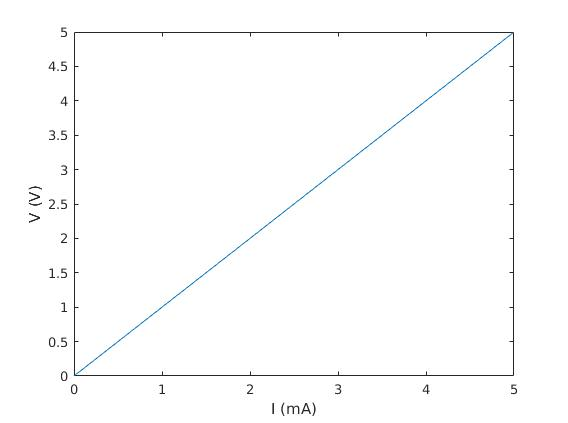
\includegraphics[width=0.65\textwidth]{img/plot1.jpg}
  \end{figure}


        
      \begin{table}[!ht]
  \captionsetup{font=large}
  \centering
  \caption{ Verification of Ohm's Law using resistor $R_2$ }
  \label{tab: ohm2 }
  \begin{tabular}{   | l | c | c | r | }
  \hline

      Source Voltage ($V_s$) &     $V_{R2}$ (V) &    $I_{R2}$ (mA)     \\ \hline
      0 &    0.0 &    0     \\ \hline
      0.5 &     0.492 &    0.224     \\ \hline
      1 &    0.992 &    0.451     \\ \hline
      1.5 &    1.493 &    0.679     \\ \hline
      2 &    1.993 &    0.906     \\ \hline
      2.5 &    2.494 &    1.134     \\ \hline
      3 &    2.995 &    1.361     \\ \hline
      3.5 &    3.493 &    1.588     \\ \hline
      4 &    3.991 &    1.814     \\ \hline
      5 &    4.990 &    2.268     \\ \hline
  
  \end{tabular}
  \end{table}



    \begin{figure}[!ht]
  \centering
  \caption{Plot of Verification of Ohm's Law using resistor $R_2$\label{fig:resultPlot2}}
  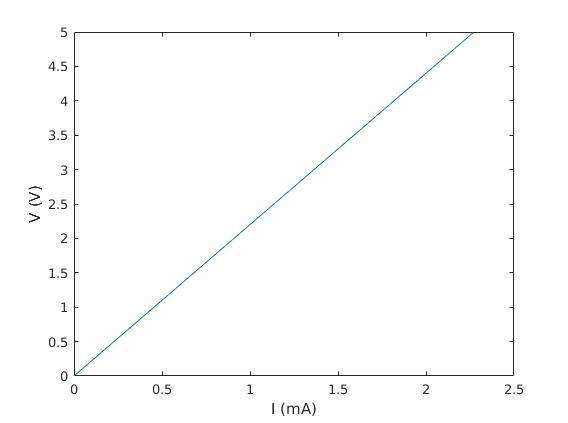
\includegraphics[width=0.65\textwidth]{img/plot2.jpg}
  \end{figure}


        
  
  
      \begin{table}[!ht]
  \captionsetup{font=large}
  \centering
  \caption{ Determination of maximum power transfer }
  \label{tab: maxpower }
  \begin{tabular}{   | l | c | c | c | c | c | r | }
  \hline

      $R_L(k \Omega)$ &     $V_L(V)$ &     $I_L(mA)$ &    $P_L$ (mW) &    $P_{in}$ (mW) &    Efficiency (\%)     \\ \hline
      6.8 &    3.78 &    0.5 &    1.89 &    2.5 &    75.6     \\ \hline
      3.3 &    2.99 &    0.86 &    2.571 &    4.3 &    59.8     \\ \hline
      2 &    2.38 &    1.14 &    2.713 &    5.7 &    47.6     \\ \hline
      1.5 &     2.00 &    1.32 &    2.64 &    6.6 &    40     \\ \hline
      1 &     1.568 &    1.51 &    2.368 &    7.55 &    31.36     \\ \hline
      0.1 &     0.217 &     2.13 &    0.462 &    10.65 &    4.34     \\ \hline
      0.047 &     0.103 &     2.19 &    0.226 &    10.95 &    2.06     \\ \hline
  
  \end{tabular}
  \end{table}



    \begin{figure}[!ht]
  \centering
  \caption{Plot of Voltage and Current as a Function of Load Resistance $R_L$\label{fig:resultCurrentvoltage}}
  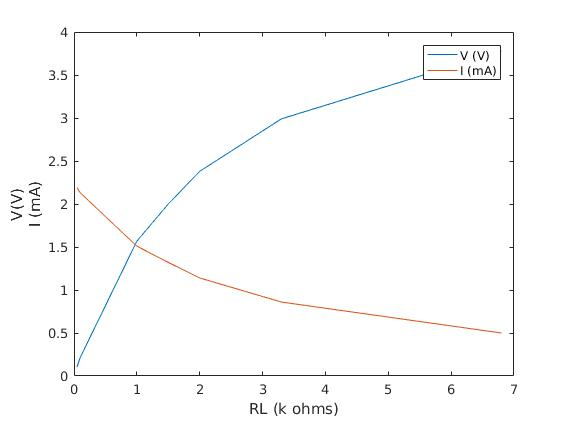
\includegraphics[width=0.75\textwidth]{img/plotc.jpg}
  \end{figure}

    \begin{figure}[!ht]
  \centering
  \caption{Plot of Load Power $P_L$ as a Function of Load Resistance $R_L$\label{fig:resultLoadpower}}
  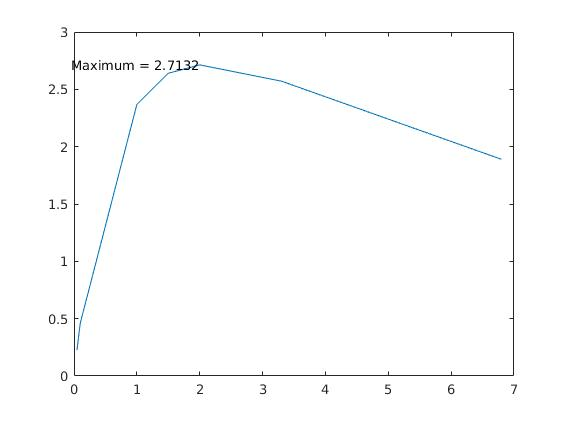
\includegraphics[width=0.7\textwidth]{img/plotd.jpg}
  \end{figure}

    \begin{figure}[!ht]
  \centering
  \caption{Plot of Efficiency $\eta$ as a Function of Load Resistance $R_L$\label{fig:resultLoadeff}}
  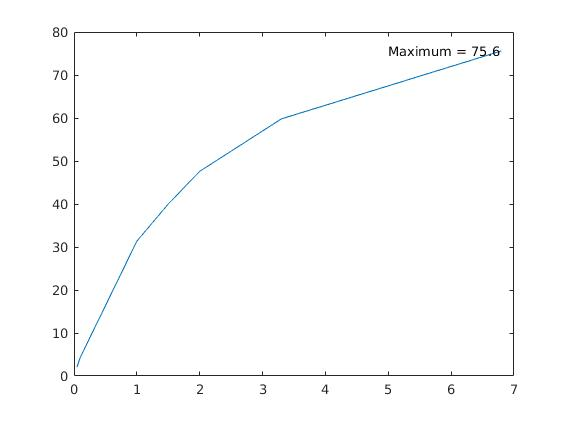
\includegraphics[width=0.7\textwidth]{img/plote.jpg}
  \end{figure}



\clearpage

\subsection{Postlab Questions}
\label{sub:Postlab Questions}

\subsubsection{Part A}

\begin{enumerate}
  \item The unknown resistors are made of linear material which can be seen from their graph.
  The graph indicates linearity by the fact that the trend line matches the
  samples points without diverging or deviating.
    \begin{figure}[!ht]
  \centering
  \caption{Verification of Ohm's Law using resistor $R_1$\label{fig:plot1}}
  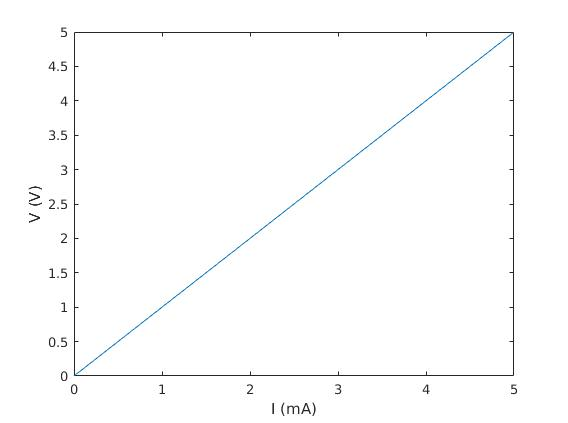
\includegraphics[width=0.65\textwidth]{img/plot1.jpg}
  \end{figure}

    \begin{figure}[!ht]
  \centering
  \caption{Verification of Ohm's Law using resistor $R_2$\label{fig:plot2}}
  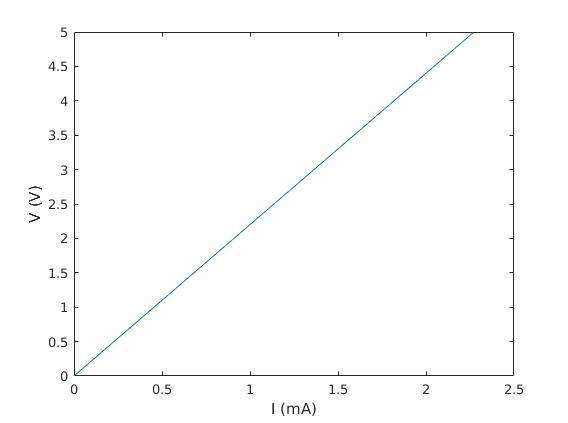
\includegraphics[width=0.65\textwidth]{img/plot2.jpg}
  \end{figure}

  \item $R_1$ and $R_2$ can be calculated by the slope of the IV graph.
  From the slope the resistances were calculated to be 1k, and 2.2k which is the
  the same as their resistance rating. Despite high accuracy there is low precision as
  the linear regression was done with a simple best fit line.
  \begin{gather}
    m = \frac{y_2-y_1}{x_2-x_1} = \frac{1.0 V - 0.0 V}{1.0 mA - 0.0 mA} = 1000 \frac{V}{A} = 1 k \Omega \\
    m = \frac{y_2-y_1}{x_2-x_1} = \frac{1.1 V - 0.0 V}{0.5 mA - 0.0 mA} = 2200 \frac{V}{A} = 2.2 k \Omega
  \end{gather}
\end{enumerate}
\vspace{1cm}
\subsubsection{Part B}
\begin{enumerate}
  \item As the load resistance increases the load voltage increases.
  There is a direct non-linear relationship between voltage and resistance. This can be seen by the blue line of plot
  figure \ref{fig:currentvoltage}. As the load resistance increases the load current decreases.
  There is a indirect non-linear relationship between current and resistance. This can be seen by the red line of the plot.\\
  The graph indicates:
  \begin{equation}
    \text{ As } R_L \to \infty \hspace{1cm} \begin{matrix}
    V_L \to V_{in} = 5 V \\
    I_L \to 0
  \end{matrix}
  \end{equation}
  Testing various resistor values in the voltage divider equation yeilds the same
  values that were measured.
  \begin{gather}
    \text{For a voltage divider: } V_{out} = V_{in} \cdot \frac{R_L}{R_S+R_L} \\
    V_{out}(R_L \to 0) = (5 V) \cdot \frac{0}{(2.2 k \Omega)+0} = 0 \\
    V_{out}(R_L \to 6.8k ) = (5 V) \cdot \frac{6.8 k \Omega}{(2.2 k \Omega)+ 6.8 k \Omega} = 3.78V
  \end{gather}



    \begin{figure}[!ht]
  \centering
  \caption{Plot of Voltage and Current as a Function of Load Resistance $R_L$\label{fig:currentvoltage}}
  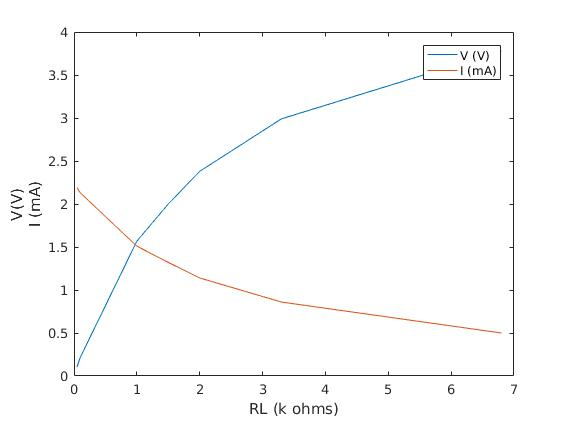
\includegraphics[width=0.75\textwidth]{img/plotc.jpg}
  \end{figure}


  \item The load power increased as the load resistance increased till it reached a maximum.
  At this point the power decreased. It created a concave down curve represented in Figure~\ref{fig:loadpower}
    \begin{figure}[!ht]
  \centering
  \caption{Plot of Load Power $P_L$ as a Function of Load Resistance $R_L$\label{fig:loadpower}}
  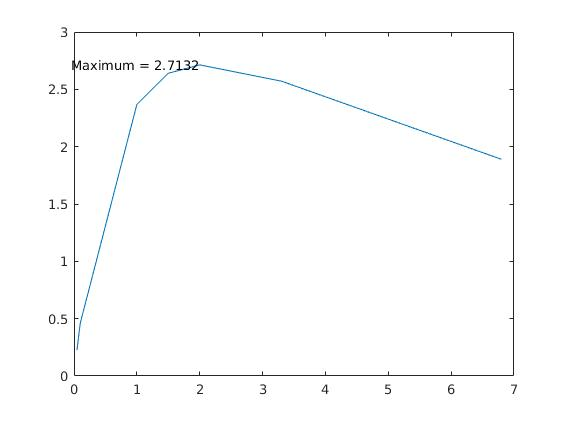
\includegraphics[width=0.7\textwidth]{img/plotd.jpg}
  \end{figure}


  \item The resistor that resulted in the maximum power transfer was the $2.0 k\Omega$
    resistor, but according to the regression of the plot (Figure~\ref{fig:loadpower}) the value would be $R_L = 2.7 k\Omega$
    Both these values fall close to the value of the source resistor which
    had a value of $R_s = 2.2 k\Omega$. To be consistent with the theorem for maximum
    power transfer the load resistor would be equal to the source resistance $R_S$.
  \item The resistor that resulted in the maximum efficiency was the $6.8k \Omega$
  resistor, but according to the regression of the plot (Figure~\ref{fig:loadeff}) the value would
  be $R_L = 75.6 k\Omega$. However, these points were the endpoints of the sample data
   and the plot respectively. In reality the maximum efficiency is only when the resistance
   reaches infinity. The end behavior of the graph indicates this by the horizontal asymptote at $100\%$.
   \[\text{As } R_L \to \infty , \eta \to 100\% \]
     \begin{figure}[!ht]
  \centering
  \caption{Plot of Efficiency $\eta$ as a Function of Load Resistance $R_L$\label{fig:loadeff}}
  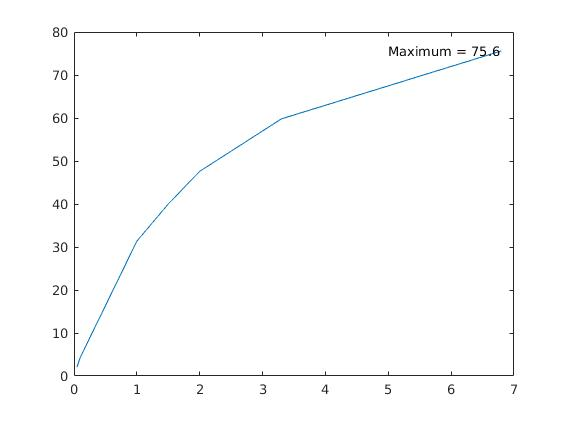
\includegraphics[width=0.7\textwidth]{img/plote.jpg}
  \end{figure}


\end{enumerate}
  \clearpage

  \section{Conclusion}
  \label{sec:Conclusion}
    \clearpage


\end{document}
